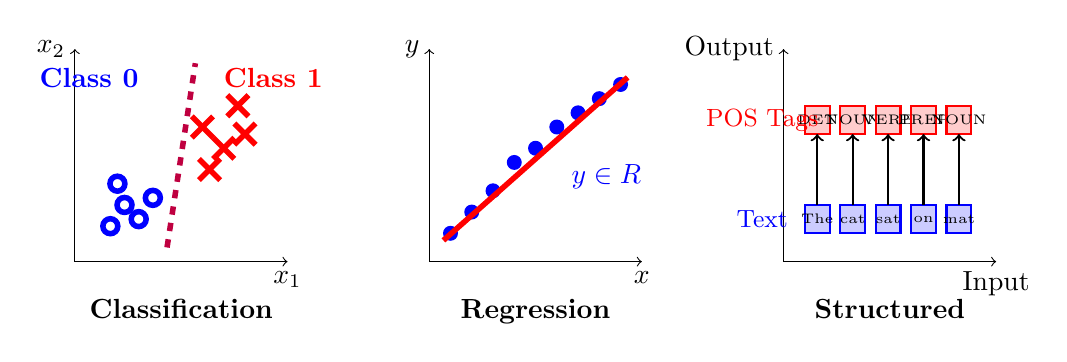
\begin{tikzpicture}[scale=0.9]
  % Classification subplot - improved
  \begin{scope}[xshift=0cm]
    \draw[->] (0,0) -- (3,0) node[below] {$x_1$};
    \draw[->] (0,0) -- (0,3) node[left] {$x_2$};
    
    % Class 1 points (circles) - larger
    \foreach \x/\y in {0.5/0.5, 0.7/0.8, 0.9/0.6, 1.1/0.9, 0.6/1.1} {
      \draw[blue, thick, line width=2pt] (\x, \y) circle (3pt);
    }
    
    % Class 2 points (crosses) - larger
    \foreach \x/\y in {1.8/1.9, 2.1/1.6, 2.3/2.2, 1.9/1.3, 2.4/1.8} {
      \draw[red, thick, line width=2pt] (\x-0.15, \y-0.15) -- (\x+0.15, \y+0.15);
      \draw[red, thick, line width=2pt] (\x-0.15, \y+0.15) -- (\x+0.15, \y-0.15);
    }
    
    % Decision boundary
    \draw[thick, purple, dashed, line width=2pt] (1.3, 0.2) -- (1.7, 2.8);
    
    \node[below] at (1.5, -0.4) {\textbf{Classification}};
    \node[blue] at (0.2, 2.6) {\textbf{Class 0}};
    \node[red] at (2.8, 2.6) {\textbf{Class 1}};
  \end{scope}
  
  % Regression subplot - improved
  \begin{scope}[xshift=5cm]
    \draw[->] (0,0) -- (3,0) node[below] {$x$};
    \draw[->] (0,0) -- (0,3) node[left] {$y$};
    
    % Continuous data points - larger
    \foreach \x/\y in {0.3/0.4, 0.6/0.7, 0.9/1.0, 1.2/1.4, 1.5/1.6, 1.8/1.9, 2.1/2.1, 2.4/2.3, 2.7/2.5} {
      \fill[blue] (\x, \y) circle (3pt);
    }
    
    % Regression line - thicker
    \draw[thick, red, line width=2pt] (0.2, 0.3) -- (2.8, 2.6);
    
    \node[below] at (1.5, -0.4) {\textbf{Regression}};
    \node[blue] at (2.5, 1.2) {$y \in \mathbb{R}$};
  \end{scope}
  
  % Structured prediction - much improved
  \begin{scope}[xshift=10cm]
    \draw[->] (0,0) -- (3,0) node[below] {Input};
    \draw[->] (0,0) -- (0,3) node[left] {Output};
    
    % Better sequence visualization
    \foreach \i/\word in {0.3/The, 0.8/cat, 1.3/sat, 1.8/on, 2.3/mat} {
      \draw[thick, blue, fill=blue!20] (\i, 0.4) rectangle +(0.35, 0.4);
      \node[font=\tiny] at (\i+0.175, 0.6) {\word};
    }
    
    \foreach \i/\tag in {0.3/DET, 0.8/NOUN, 1.3/VERB, 1.8/PREP, 2.3/NOUN} {
      \draw[thick, red, fill=red!20] (\i, 1.8) rectangle +(0.35, 0.4);
      \node[font=\tiny] at (\i+0.175, 2.0) {\tag};
    }
    
    % Arrows showing mapping
    \foreach \i in {0.475, 0.975, 1.475, 1.975, 2.475} {
      \draw[thick, ->] (\i, 0.8) -- (\i, 1.8);
    }
    
    \node[below] at (1.5, -0.4) {\textbf{Structured}};
    \node[blue, font=\small] at (-0.3, 0.6) {Text};
    \node[red, font=\small] at (-0.3, 2.0) {POS Tags};
  \end{scope}
\end{tikzpicture}
